\section{Diseño y Construcción de la Computadora de Vuelo}

% ==============================================
\begin{frame}{Objetivos}
	\begin{enumerate}
		\item<2->Incorporar interfaz de comunicación dedicada a la tolerancia a fallas.
		\item<3->Actualizar componentes.
		\item<4->Incorporar conectores necesarios para integración de sensores y módulos externos.
		\item<5->Mantener las dimensiones reducidas.
	\end{enumerate}
\end{frame}

% ==============================================
\begin{frame}{Antecedentes}
	\begin{itemize}
		\item <1->En el Laboratorio de Automática y Robótica (LAR) se han desarrollado computadoras de vuelo.
	\end{itemize}
	\begin{center}
		\begin{overprint}
			\onslide<2>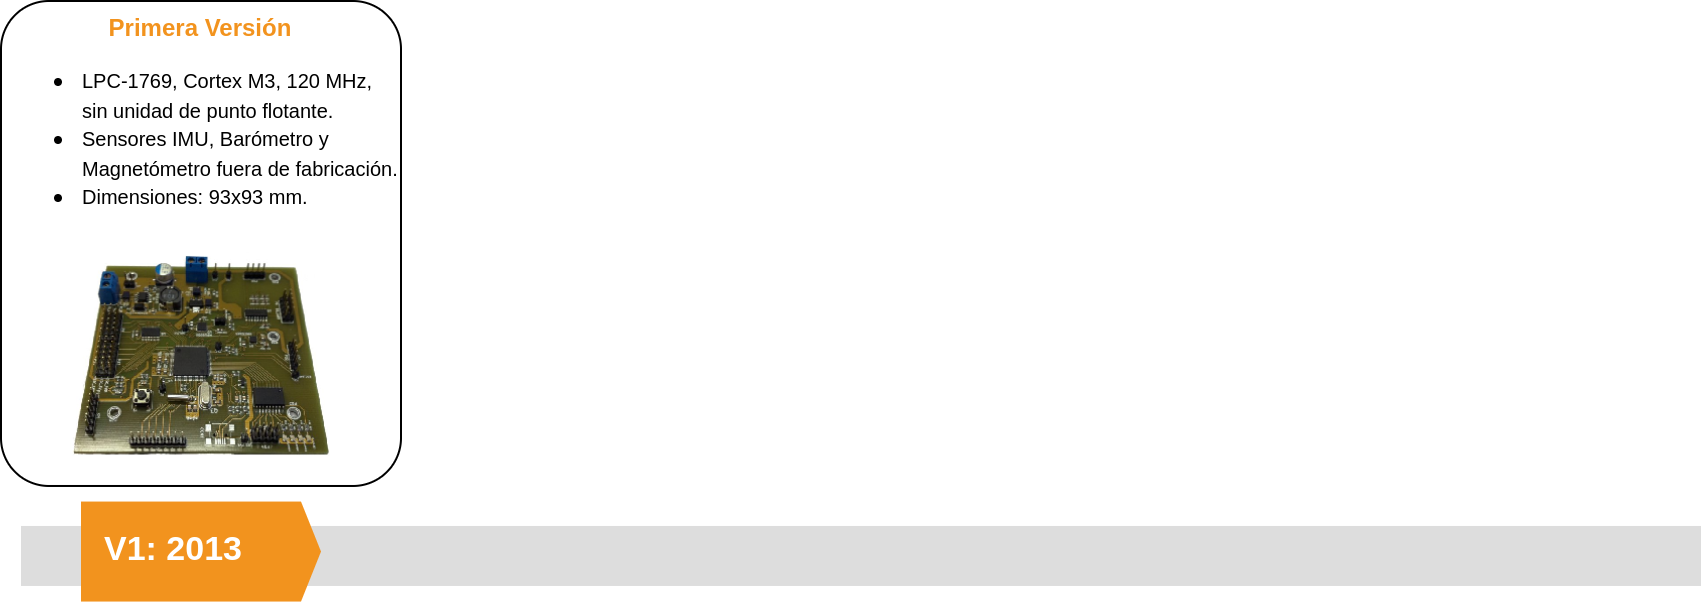
\includegraphics[width=\textwidth]{img/antecedentes_1.png}
			\onslide<3>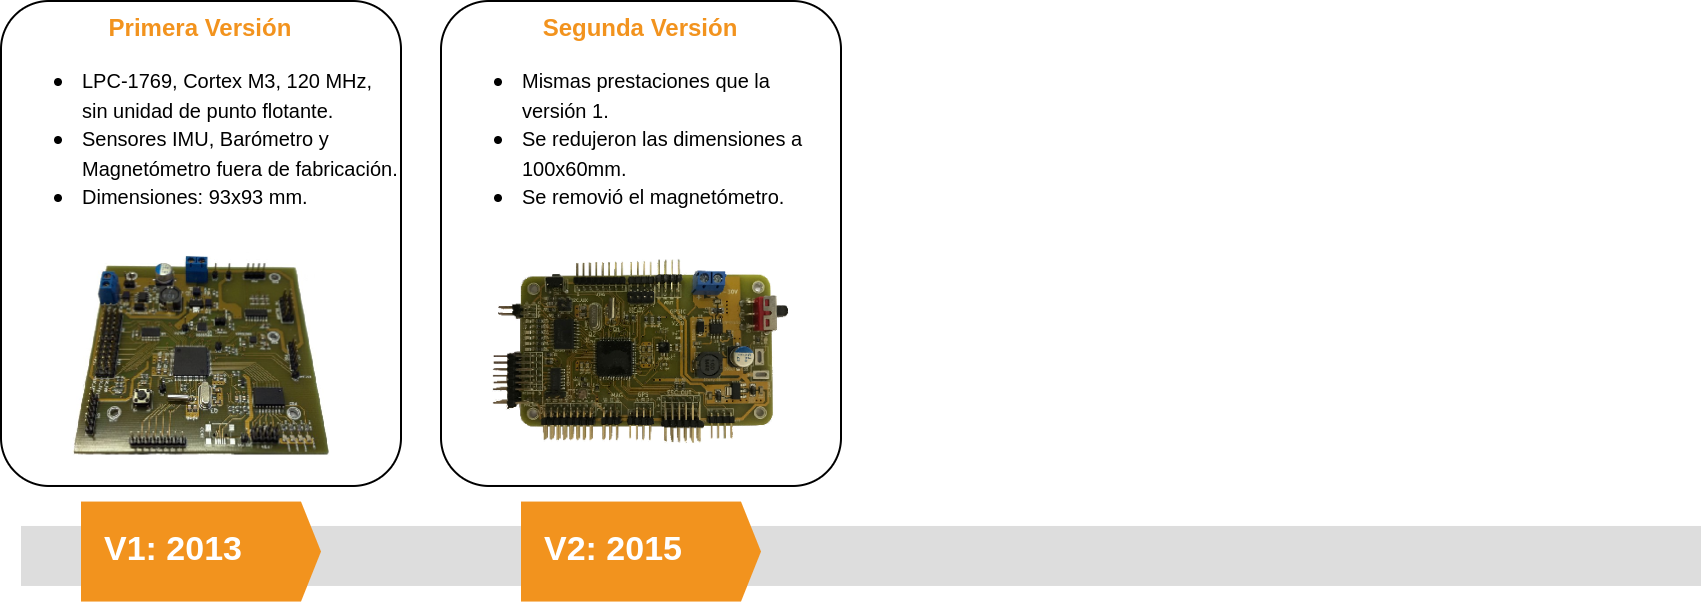
\includegraphics[width=\textwidth]{img/antecedentes_2.png}
			\onslide<4>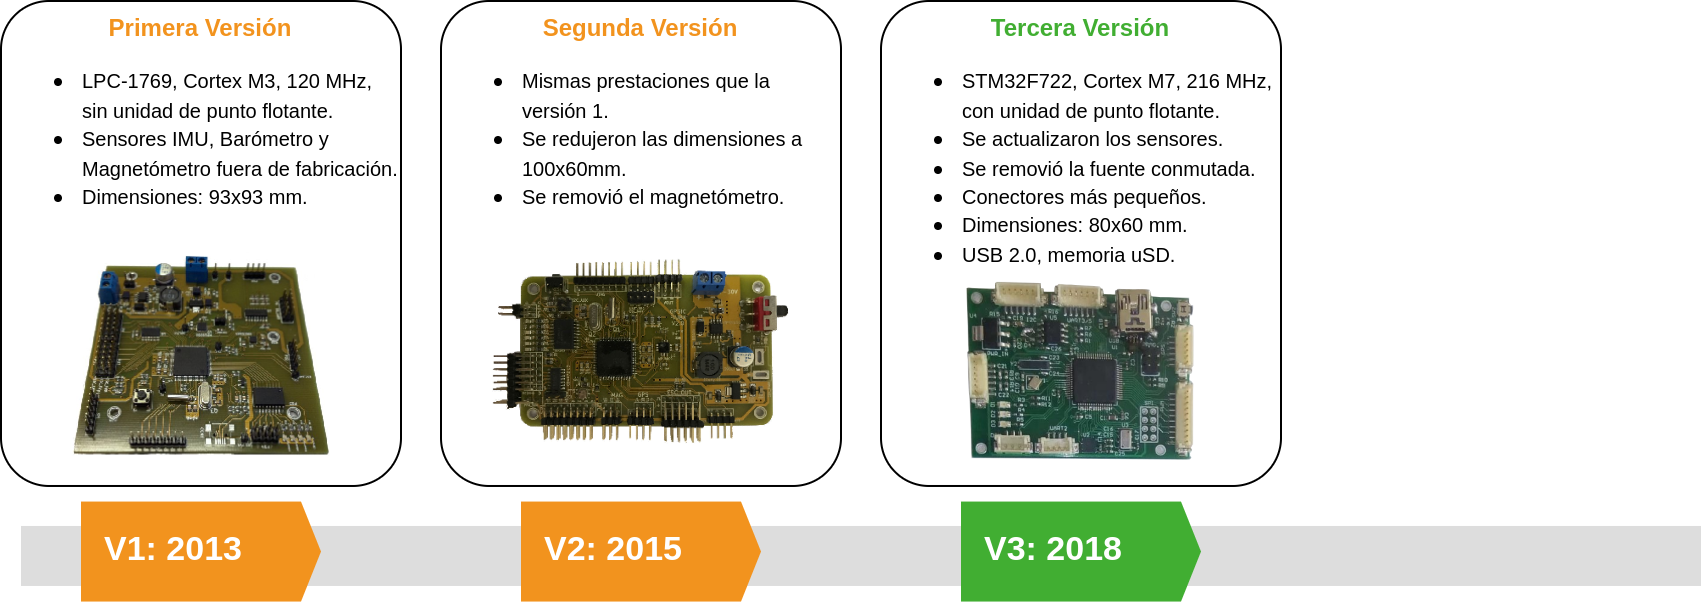
\includegraphics[width=\textwidth]{img/antecedentes_3.png}
			\onslide<5>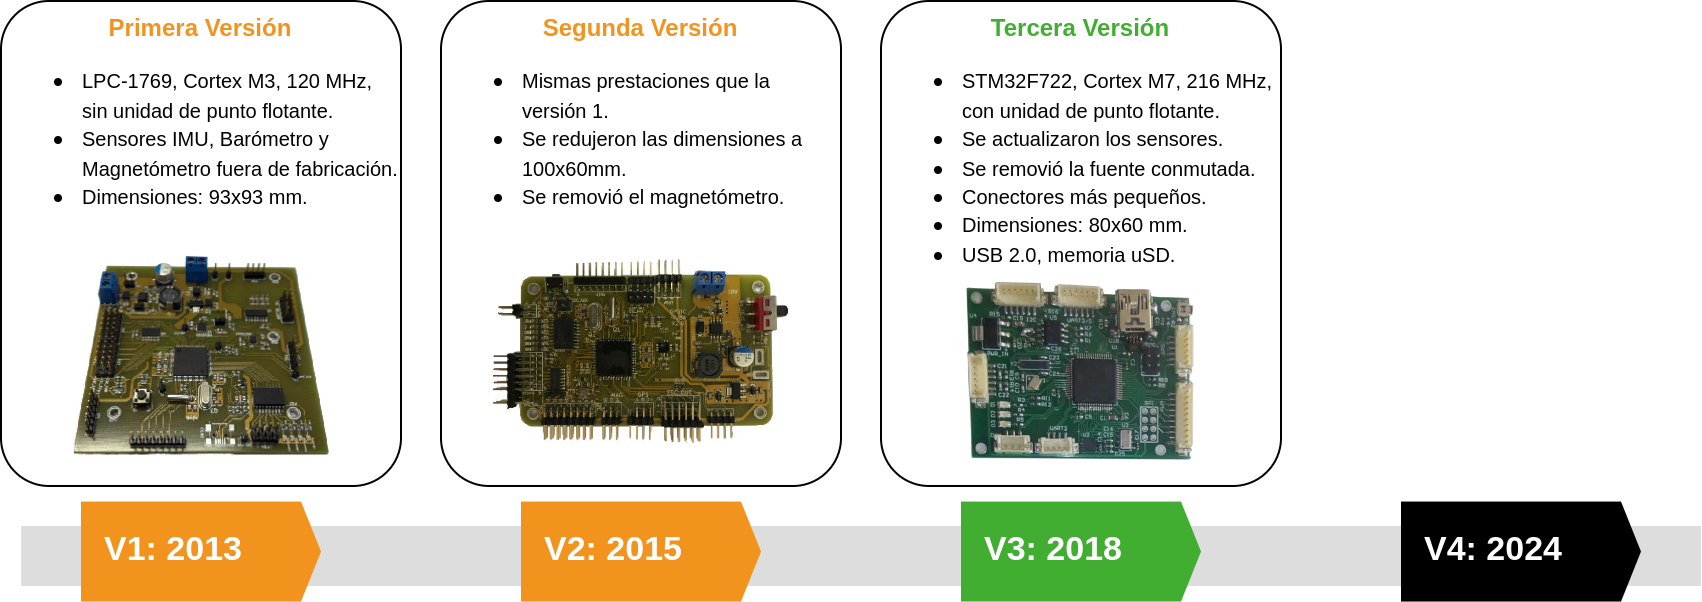
\includegraphics[width=\textwidth]{img/antecedentes_4.png}
		\end{overprint}
	\end{center}
\end{frame}

% ==============================================
\begin{frame}{Componentes y Funcionalidades}
	\begin{columns}
		\column{0.4\textwidth}
			\begin{center}
				\onslide<2->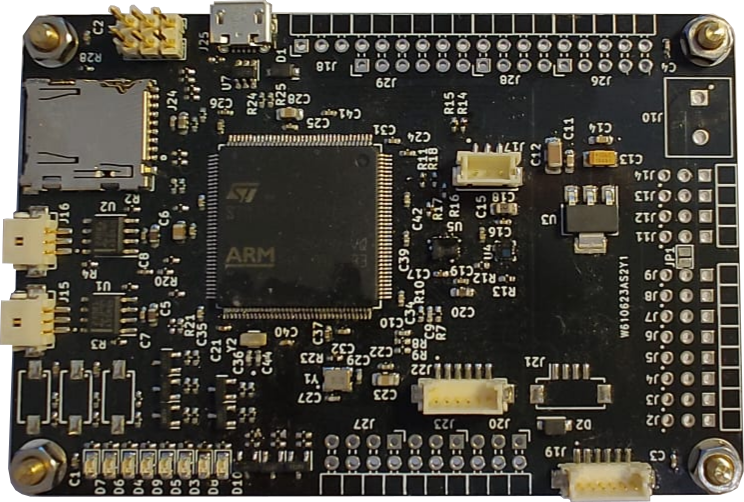
\includegraphics[width=\textwidth]{img/Choriboard_IV.png}\\
				\vspace{0.6cm}
				\onslide<1->
\includegraphics[width=\textwidth]{img/cosito_2_V4.png}
			\end{center}
		\column{0.6\textwidth}
			\begin{itemize}
				\item<3->Microcontrolador STM32F746ZG, Cortex M7, 216 MHz.
				\item<4->Sensores: IMU y Barómetro (magnetómetro externo).
				\item<5->Interfaz CAN x2.
				\item<6->Interfaces varias: UART, SPI, I2C, USB, DSM Spektrum y PPM.
				\item<7->Slot para memoria uSD.
				\item<8->PCB de 4 capas, diseñado usando KiCad.
				\item<9->Todos los componentes en una sola cara.
				\item<10->Se fabricaron 3 placas.
			\end{itemize}
	\end{columns}
\end{frame}

% ==============================================
\begin{frame}{Microcontrolador}
	\begin{columns}
		\column{0.4\textwidth}
			\begin{center}
				%\onslide<2->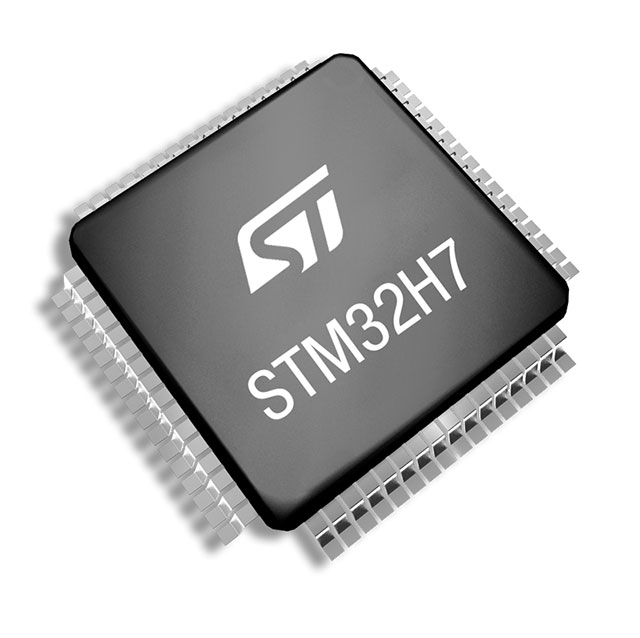
\includegraphics[width=\textwidth]{img/STM32H7_series.jpg}
				\onslide<2->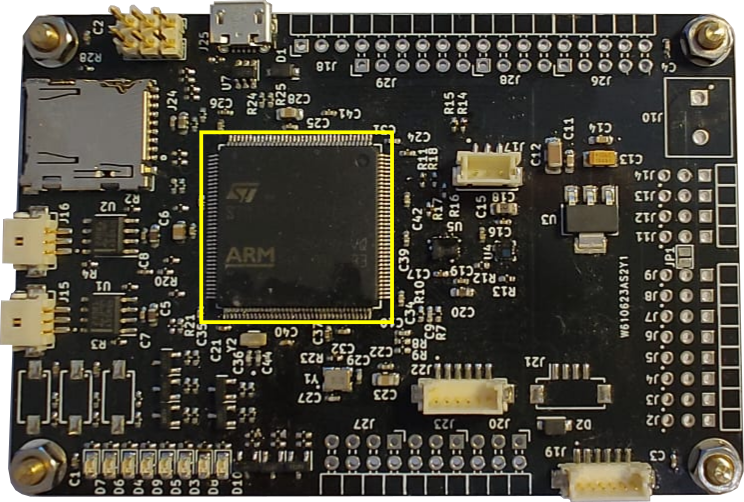
\includegraphics[width=\textwidth]{img/microcontrolador.png}
			\end{center}
		\column{0.6\textwidth}
			\begin{itemize}
				\item<2-> Mejorar la performance.
				\item<3-> Tener retrocompatibilidad con el firmware de la V3.
				\item<4-> Serie STM32H7: Cortex M7, 550 MHz, longevidad 10 años.
				\item<5-> La selección final se vio afectada por el faltante de componentes en 2022, ninguno de la serie STM32H7 se encontraba disponible.
				\item<6-> Se seleccionó un modelo similar al anterior: STM32F746ZG.
				\item<7-> Flash: 1024 kB, SRAM: 320 kB.
 				\item<7-> Longevidad 10 años, hasta enero 2034.
 				\item<7-> En la actualidad se reemplazó por el STM32F777ZIT6, compatible pin a pin.
				\end{itemize}
	\end{columns}
\end{frame}

% \begin{frame}{Microcontrolador}
% 	\begin{columns}
% 		\column{0.4\textwidth}
% 			\begin{center}
% 				\onslide<2->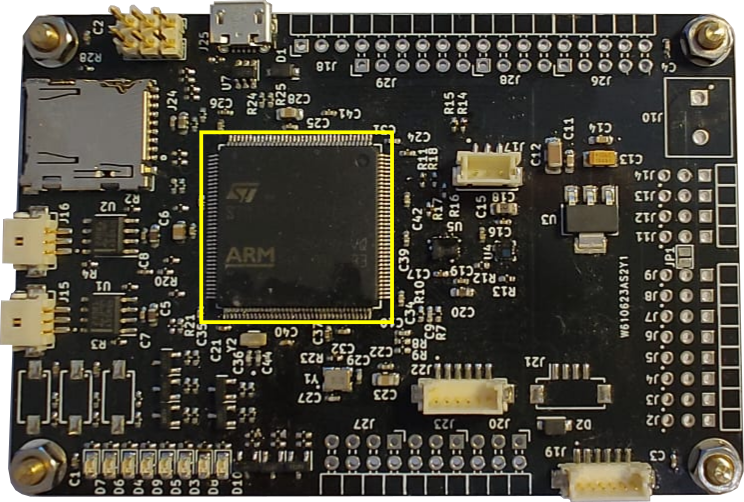
\includegraphics[width=\textwidth]{img/microcontrolador.png}
% 			\end{center}
% 		\column{0.6\textwidth}
% 			\begin{itemize}
% 				\item La selección final se vio afectada por el faltante de componentes en 2022, ninguno de la serie STM32H7 se encontraba disponible.
% 				\item Se seleccionó un modelo similar al anterior: STM32F746ZG.
% 				\item Flash: 1024 kB, SRAM: 320 kB.
% 				%\item Longevidad 10 años, hasta enero 2034.
% 				\item En la actualidad se reemplazó por el STM32F777ZIT6, compatible pin a pin.
% 				\item Tiene unidad de punto flotante de doble precisión.
% 			\end{itemize}
% 	\end{columns}
% \end{frame}

% ==============================================
\begin{frame}{Unidad de Medición Inercial (IMU)}
	% \begin{itemize}
	% 	\item Modelo ICM42688p, del mismo fabricante de la V3.
	% 	\item Tener reutilización del firmware.
	% 	\item Menor ruido y error de factor de escala para giróscopos.
	% \end{itemize}
	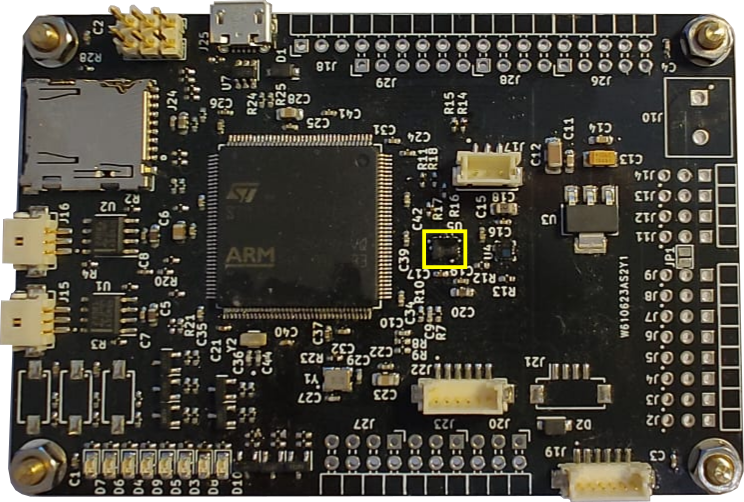
\includegraphics[width=0.5\textwidth]{img/IMU.png}
	COMPLETAR CON UNA FOTO HACIENDO ZOOM A LA IMU PARA QUE SE VEA QUE ES MUY PEQUEÑA.
\end{frame}

\begin{frame}{Unidad de Medición Inercial (IMU)}
	\begin{itemize}
		\item Acelerómetros y giróscopos triaxiales.
		\item Permite medir aceleración lineal y velocidad angular en una terna solidaria al componente.
		\item El sensor principal para mantener la estabilidad del vehículo.
		\item Las mediciones pueden utilizarse para estimar la orientación del vehículo respeto de una terna inercial.
	\end{itemize}
\end{frame}

\begin{frame}{Unidad de Medición Inercial (IMU)}
	\begin{itemize}
		\item Se hizo una búsqueda de alternativas.
		\item Especificaciones más relevantes:
		\begin{itemize}
			\item Variación del offset con el tiempo de acelerómetros.
			\item Variación del offset con el tiempo de giróscopos.
			\item Error factor de escala de giróscopos.
			\item Ruido de giróscopos.
		\end{itemize}
		\item Sin embargo de todas las alternativas, solo 1 de ellas tenía una hoja con todas las especificaciones.
	\end{itemize}
	\begin{columns}
		\column{0.4\textwidth}
			\begin{center}
				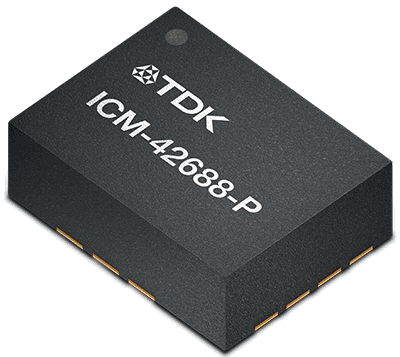
\includegraphics[width=0.5\textwidth]{img/icm42688p.png}
			\end{center}
		\column{0.6\textwidth}
			\begin{itemize}
			 	\item Modelo ICM42688p, del mismo fabricante de la V3.
				\item Tener reutilización del firmware.
		 		\item Menor ruido y error de factor de escala para giróscopos.
			\end{itemize}
	\end{columns}
\end{frame}



% \begin{frame}{Unidad de Medición Inercial (IMU)}
% 	\begin{itemize}
% 		\item<1-> Las hojas de datos muestran una gran cantidad de especificaciones, tanto para los acelerómetros como para los giróscopos.
% 		\item<3-> Se tomaron como referencia un set reducido de las especificaciones.
% 		\item<4-> Estas tienen impacto en las estimaciones de posición y orientación.
% 	\end{itemize}
% 	%\vspace{0.5cm}
% 	\onslide<2->\begin{table}
% 		\centering
% 		\begin{tabular}{|c||c|}
% 			\hline
% 	    	Acelerómetros & Giróscopos\\
% 	    	\hline
% 	    	Full-scale range & Full-scale range\\
% 	    	Scale factor error & Scale factor error\\
% 	    	Scale factor error vs temperature & Scale factor error vs temperature\\
% 	    	Offset & Offset\\
% 	    	Offset vs temperature & Offset vs temperature\\
% 	    	Offset vs time & Offset vs time\\
% 	    	Noise & Noise\\
% 	    	\hline
% 	    \end{tabular}
% 	\end{table}
% \end{frame}

% \begin{frame}{Unidad de Medición Inercial (IMU)}
% 	\begin{itemize}
% 		\item Las hojas de datos muestran una gran cantidad de especificaciones, tanto para los acelerómetros como para los giróscopos.
% 		\item Se tomaron como referencia un set reducido de las especificaciones.
% 		\item Estas tienen impacto en las estimaciones de posición y orientación.
% 	\end{itemize}
% 	%\vspace{0.5cm}
% 	\begin{table}
% 		\centering
% 		\begin{tabular}{|c||c|}
% 			\hline
% 	    	Acelerómetros & Giróscopos\\
% 	    	\hline
% 	    	Full-scale range & Full-scale range\\
% 	    	Scale factor error & \textbf{Scale factor error}\\
% 	    	Scale factor error vs temperature & Scale factor error vs temperature\\
% 	    	Offset & Offset\\
% 	    	Offset vs temperature & Offset vs temperature\\
% 	    	\textbf{Offset vs time} & \textbf{Offset vs time}\\
% 	    	Noise & \textbf{Noise}\\
% 	    	\hline
% 	    \end{tabular}
% 	\end{table}
% \end{frame}

% ==============================================
\begin{frame}{Barómetro}
	\begin{columns}
		\column{0.4\textwidth}
			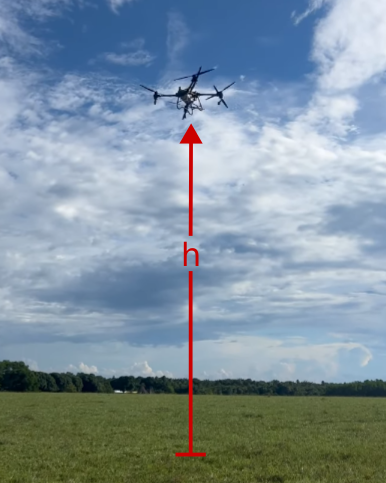
\includegraphics[width=0.7\textwidth]{img/drone_altitude.png}
			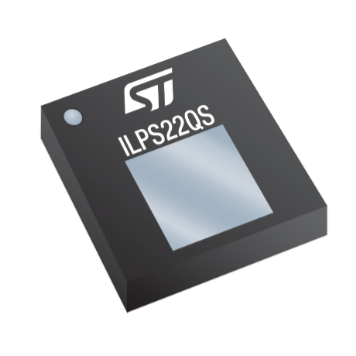
\includegraphics[width=0.6\textwidth]{img/ILSP22QSTR.png}
		\column{0.6\textwidth}
			\begin{itemize}
				\item Se utiliza para medir diferencias de presión atmosférica, lo que permite medir diferencias de altura.
				\item Especificación de interés: exactitud relativa.
				\item Componente seleccionado: ILPS22QSTR.
			\end{itemize}
	\end{columns}
\end{frame}

% ==============================================
\begin{frame}{Magnetómetro}

\end{frame}

% ==============================================
\begin{frame}{Interfaz CAN}

\end{frame}

% ==============================================
\begin{frame}{Alimentación} %Explicar acá mismo lo del PCB

\end{frame}

% ==============================================
\begin{frame}{Interfaz uSD} %Explicar acá mismo lo del PCB

\end{frame}

% ==============================================
\begin{frame}{Interfaz USB} %Explicar acá mismo lo del PCB

\end{frame}

% ==============================================
\begin{frame}{Montaje} %Foto de las placas stackeadas

\end{frame}